\documentclass[11pt, a4paper, twoside]{article} %draft

\usepackage{url}
\usepackage{amsmath}
\usepackage{graphicx}
\usepackage{array}
\usepackage{babel,csquotes,xpatch}
\usepackage[backend=bibtex8]{biblatex}
\usepackage{nameref}
\usepackage{xcolor}
\usepackage{tikz}
\usetikzlibrary{arrows,automata}
\usepackage{dirtree}
\usepackage{listings}
\usepackage{packages/listings-golang}
\usepackage{enumitem}

\lstset{
	frame=tb,
	tabsize=4,
	numbers=left,
	numberstyle=\tiny\color{gray},
	basicstyle=\footnotesize
}

%define Javascript language
\lstdefinelanguage{JavaScript}{
	keywords={typeof, new, true, false, catch, function, return, null, catch, switch, var, if, in, while, do, else, case, break},
	keywordstyle=\color{blue}\bfseries,
	ndkeywords={class, export, boolean, throw, implements, import, this, require},
	ndkeywordstyle=\color{darkgray}\bfseries,
	identifierstyle=\color{black},
	sensitive=false,
	comment=[l]{//},
	morecomment=[s]{/*}{*/},
	commentstyle=\color{purple}\ttfamily,
	stringstyle=\color{red}\ttfamily,
	morestring=[b]',
	morestring=[b]"
}



%main colors of CP-MAC app
\definecolor{accent-light}{RGB}{192, 204, 217}
\definecolor{accent-dark}{RGB}{129, 144, 164}

% used to create a square of 0.3cm x 0.3cm to show solor palettes
\newcommand\crule[1][black]{\textcolor{#1}{\rule{0.3cm}{0.3cm}}}


\addbibresource{resources/bibliography.bib}



\begin{document}
% Example of title page for the projects carried out within DEDIS
% Copied from lasec 

% Simply include it in your mastex tex file: 
%        % Example of title page for the projects carried out within DEDIS
% Copied from lasec 

% Simply include it in your mastex tex file: 
%        % Example of title page for the projects carried out within DEDIS
% Copied from lasec 

% Simply include it in your mastex tex file: 
%        \input{cover}


% Updated October 2016


\newcommand{\logoepfl}[0]{
  \begin{center}
    
\includegraphics[width=4cm]{logo_epfl_coul.eps}
  \end{center}
  \vspace{0.3cm}
  \hrule
}
\newcommand{\project}[1]{
  \begin{center}
    \large{#1}
  \end{center}
  \vspace{1cm}
}
\newcommand{\department}[1]{
  \begin{center}
    \large{#1}
  \end{center}
}
\newcommand{\lab}[1]{
  \begin{center}
    \large{#1}
  \end{center}
}
\newcommand{\supervisor}[3]{
  \begin{center}
    \begin{normalsize}{
        \bf #1}\\#2\\#3
    \end{normalsize}
  \end{center}
}
\renewcommand{\author}[1]{
  \begin{center}
    \Large{#1}
  \end{center}
  \vspace{0.5cm}
}
\renewcommand{\title}[1]{
  \vspace{3cm}
  \begin{center}
    \huge{#1}
  \end{center}
  \vspace{1.7cm}
}
\renewcommand{\date}[2]{
  \begin{center}
    \normalsize{#1 #2}
  \end{center}
  \vspace{0.5cm}
}


\thispagestyle{empty}


% begin title page
  \logoepfl
  
  \title{Cross-Platform Mobile Application for the Cothority}
  
  \author{Cedric Maire}
  \department{School of Computer and Communication Sciences}
  \lab{Decentralized and Distributed Systems Lab}
  \project{Semester Project}
  
  \date{January}{2018}

  \begin{center}
    \begin{tabular}{cc}
      \begin{tabular}{p{4.0cm}}
        \supervisor{Responsible}{Prof. Bryan Ford}{EPFL / DeDiS}
      \end{tabular}&
      \begin{tabular}{p{4.0cm}}
        \supervisor{Supervisor}{Linus Gasser}{EPFL / DeDiS}
      \end{tabular}
    \end{tabular}
  \end{center}

% end title page



% Updated October 2016


\newcommand{\logoepfl}[0]{
  \begin{center}
    
\includegraphics[width=4cm]{logo_epfl_coul.eps}
  \end{center}
  \vspace{0.3cm}
  \hrule
}
\newcommand{\project}[1]{
  \begin{center}
    \large{#1}
  \end{center}
  \vspace{1cm}
}
\newcommand{\department}[1]{
  \begin{center}
    \large{#1}
  \end{center}
}
\newcommand{\lab}[1]{
  \begin{center}
    \large{#1}
  \end{center}
}
\newcommand{\supervisor}[3]{
  \begin{center}
    \begin{normalsize}{
        \bf #1}\\#2\\#3
    \end{normalsize}
  \end{center}
}
\renewcommand{\author}[1]{
  \begin{center}
    \Large{#1}
  \end{center}
  \vspace{0.5cm}
}
\renewcommand{\title}[1]{
  \vspace{3cm}
  \begin{center}
    \huge{#1}
  \end{center}
  \vspace{1.7cm}
}
\renewcommand{\date}[2]{
  \begin{center}
    \normalsize{#1 #2}
  \end{center}
  \vspace{0.5cm}
}


\thispagestyle{empty}


% begin title page
  \logoepfl
  
  \title{Cross-Platform Mobile Application for the Cothority}
  
  \author{Cedric Maire}
  \department{School of Computer and Communication Sciences}
  \lab{Decentralized and Distributed Systems Lab}
  \project{Semester Project}
  
  \date{January}{2018}

  \begin{center}
    \begin{tabular}{cc}
      \begin{tabular}{p{4.0cm}}
        \supervisor{Responsible}{Prof. Bryan Ford}{EPFL / DeDiS}
      \end{tabular}&
      \begin{tabular}{p{4.0cm}}
        \supervisor{Supervisor}{Linus Gasser}{EPFL / DeDiS}
      \end{tabular}
    \end{tabular}
  \end{center}

% end title page



% Updated October 2016


\newcommand{\logoepfl}[0]{
  \begin{center}
    
\includegraphics[width=4cm]{logo_epfl_coul.eps}
  \end{center}
  \vspace{0.3cm}
  \hrule
}
\newcommand{\project}[1]{
  \begin{center}
    \large{#1}
  \end{center}
  \vspace{1cm}
}
\newcommand{\department}[1]{
  \begin{center}
    \large{#1}
  \end{center}
}
\newcommand{\lab}[1]{
  \begin{center}
    \large{#1}
  \end{center}
}
\newcommand{\supervisor}[3]{
  \begin{center}
    \begin{normalsize}{
        \bf #1}\\#2\\#3
    \end{normalsize}
  \end{center}
}
\renewcommand{\author}[1]{
  \begin{center}
    \Large{#1}
  \end{center}
  \vspace{0.5cm}
}
\renewcommand{\title}[1]{
  \vspace{3cm}
  \begin{center}
    \huge{#1}
  \end{center}
  \vspace{1.7cm}
}
\renewcommand{\date}[2]{
  \begin{center}
    \normalsize{#1 #2}
  \end{center}
  \vspace{0.5cm}
}


\thispagestyle{empty}


% begin title page
  \logoepfl
  
  \title{Cross-Platform Mobile Application for the Cothority}
  
  \author{Cedric Maire}
  \department{School of Computer and Communication Sciences}
  \lab{Decentralized and Distributed Systems Lab}
  \project{Semester Project}
  
  \date{January}{2018}

  \begin{center}
    \begin{tabular}{cc}
      \begin{tabular}{p{4.0cm}}
        \supervisor{Responsible}{Prof. Bryan Ford}{EPFL / DeDiS}
      \end{tabular}&
      \begin{tabular}{p{4.0cm}}
        \supervisor{Supervisor}{Linus Gasser}{EPFL / DeDiS}
      \end{tabular}
    \end{tabular}
  \end{center}

% end title page


\clearpage

\thispagestyle{empty}
\subsection*{Acknowledgments}
I would like to thank Linus Gasser who gave me the chance to do this project. I would also like to thank him for the help he provided me all along the semester, which gave me the confidence to go through the different challenges this project imposed. Beside giving me a lot of new knowledge on  cryptography subjects , this project strengthens my belief of continuing my studies in the field of decentralized technologies. I would also like to thank Gaurav Gnarula, in charge of the CothorityJS and KyberJS modules, who provides me a valuable help to resolve the bugs related to their execution in the NativeScript environment. Finally, I would like to thank the \textit{Blockchain Society}\footnote{\url{https://blockchainsociety.ch}} for their patience during the two sessions of real-world testing of CP-MAC.

\clearpage

\tableofcontents{\protect\thispagestyle{empty}

\clearpage


% Start page count
\setcounter{page}{1}

\section{Introduction}
In this report, I will present the work that has been done on the CP-MAC cross-platform mobile application. CP-MAC allows a user to use the framework Cothority, developed at the DEDIS lab, in a functional and user-friendly application. The base application containing all the primitives to use the framework was already done during a previous semester project, thus the focus in this project was to improve the user experience and to extend the application with a new functionality. The chosen functionality is the BeerCoin, a long time running joke at the DEDIS lab which consists of beer tokens that can be distributed in a group using Proof-Of-Personhood. A token can then be used to get a beer and the barman can cryptographically verify if this token is part of the allowed group and unused.

\chapter{Background}
\section{Cothority}

\paragraph{}
The Cothority framework is composed of multiple protocols, services, and apps. At its current stage of development, CPMAC only supports the CISC and PoP apps, but it is intended to progressively feature and integrate more apps. We now present these two apps in more depth.

\subsection{CISC}

CISC stands for Cothority Identity SkipChain. The goal of this application is to provide a simple way to store data. It is based on Identity SkipChains which are permissioned blockchain-based key/value storages for organizing identities (e.g., SSH-keys). The main use of the Cisc is to store data so that it is easy to modify/add/remove it if you have a majority of the registered device in your control. This way, if the user lose a device or one of his device gets stolen, he won't lose the data, and no harm can be done. Here are some of the terms that will be used throughout this paper:
\begin{description}[style=nextline]
\item[SkipChain] A very simple, extendable voting-based permissioned blockchain based on the Chainiac-paper. In the cisc implementation, users use a personal blockchain to store there data.
\item[Data] The data stored on the Cisc SkipChain can either be SSH-public keys, web pages or any key-value pairs.
\item[Manager] The owner of the SkipChain.
\item[Device] A laptop, a smartphone... Basicaly anything the manager owns that could connect to its skipchain. In this paper we will talk about computers and smartphones.
\end{description}

\subsection{PoP}

\paragraph{}
The PoP app of the cothority framework is used to generate and verify proof of personhood, which indicates that a user is a human being. Personhood is proven through stating that a specific person was at a precise location at a particular time and thus that this user is not a bot or any other kind of human-simulating program. Before continuing, we define some important terms.

\begin{description}[style=nextline]
\item[Key Pair] In cryptography a key pair is composed of a public and private key, the public key is shared with anyone as opposed to the private key which has to remain secret to the owner of the key pair. Typically a message is decrypted and/or signed with the private key and can then be encrypted and/or verified with the public key.

\item[Conode Linking] Before being able to exchange data with a cothority node, one has to link itself to it, this is done by registering the public key on the conode after having shown that one has access to it (typically by reading a short PIN in the server logs).

\item[PoP Party] A PoP party is a gathering of people wanting to prove that they are human beings by showing everyone that they are able to come to a specific location at a specific time.

\item[Organizer (Org)] An organizer is someone hosting a PoP party by providing a conode. Since there are multiple organizers, their conodes form a cothority network and thus host the party in a distributed and decentralized manner.

\item[Attendee (Att)] An attendee is someone present at a PoP party without providing a conode and thus only attending it for the sake of a PoP token (an organizer can at the same time be an attendee).

\item[PoP Party Configuration/Description (Config/Desc)] The configuration or description of a PoP party defines all the required properties. It should include the name, the date and time, the location and a list of all the hosting conodes (which is commonly refered to as a roster) for the PoP party.

\item[Attendee Registration] The attendee registration is the process of registering all the public keys of the attendees on each of the organizers conodes, all the organizers have to do it separately for their own server.

\item[Final Statement] A final statement of a PoP party is generated by the cothority network composed of the hosting conodes, it is composed of a PoP party configuration, all the public keys of the attendees, the collective signature generated by the hosting conodes and a boolean to state if this PoP party has been merged with another one.

\item[PoP Token] A PoP token is the final token proving that the holder is a human being and attended this particular PoP party, it is composed of a final statement and a key pair.
\end{description}

\paragraph{}
First, all of the party organisers must agree on a date, time, and location. Once these specifications are set, all of the attendees (including the organisers) meet at the right location, date, and time. Each organiser has to link with a conode, complete the PoP configuration, and register it on his or her own conode; the organisers then receive the identification of this PoP party, which is henceforth used as a reference to uniquely identify it. Once every organiser registered the configuration and the PoP party is over, each one registers the list of all of the public keys of the attendees. During this step, the organisers have to ensure that each attendee has registered one and only one public key; this is a crucial step because otherwise an attendee could generate PoP tokens for every public key that he or she registered. This would then contradict the important criterion that each human being is unique and thus should only receive one PoP token for each attended party. Once every organiser registered all of the attendees, the cothority composed of their conodes finalises the party by generating the final statement containing all relevant information, which includes a collective signature. This final statement is then sent to the attendees so that they can generate their PoP token by linking this final statement to their key pair.

\section{Technologies}

\paragraph{}
Throughout this project many different technologies were used, we are now quickly presenting the main ones in a few words.

\pagebreak
\subsection[Elliptic Curve Cryptography]{Elliptic Curve Cryptography\raisebox{.3\baselineskip}{\normalsize\footnotemark}}
\footnotetext{\url{https://en.wikipedia.org/wiki/Elliptic-curve_cryptography}}

\paragraph{}
This public-key cryptographic system using elliptic curves (EC) has been independently suggested by Neal Koblitz and Victor S. Miller in 1985. EC algorithms only entered wide use in 2004 to 2005. The major difference with prior cryptographic protocols (for example DSA or RSA), that were defined over multiplicative groups of finite fields, is that EC cryptography uses point addition instead of modular exponentiation. This results in faster computation.

\subsection[Schnorr Signature]{Schnorr Signature\raisebox{.3\baselineskip}{\normalsize\footnotemark}}
\footnotetext{\url{https://en.wikipedia.org/wiki/Schnorr_signature}}

\paragraph{}
The schnorr signature algorithm is considered as one of the simplest scheme being provably secure in a random oracle model to produce digital signatures. In addition to that, the schnorr algorithm is efficient and produces short signatures.

\subsection[Protocol Buffers]{Protocol Buffers\raisebox{.3\baselineskip}{\normalsize\footnotemark}}
\footnotetext{\url{https://en.wikipedia.org/wiki/Protocol_Buffers}}

\paragraph{}
Developed by Google, this data interchange format is a language- and platform-neutral structured data serializer. Protobuf allows to define data structures once and then easily write to or read from data streams. In this particular project it is used to encode JS objects and decode byte streams received from the conodes and thus ease the process of data exchange.

\subsection[Websocket]{Websocket\raisebox{.3\baselineskip}{\normalsize\footnotemark}}
\footnotetext{\url{https://en.wikipedia.org/wiki/WebSocket}}

\paragraph{}
This communication protocol uses a single TCP connection to send data back and forth while keeping the connection open, thus facilitates real-time data transfers from and to the server. It is the used protocol for data exchange with the conodes.

\begin{figure}[h]
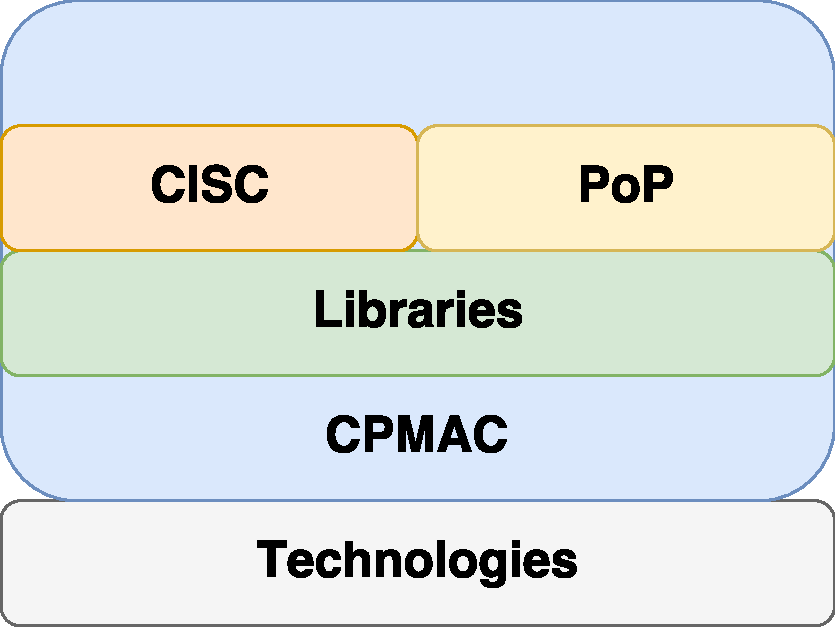
\includegraphics[scale=.3]{graphic/cpmac.pdf}
\centering
\caption{CPMAC Structure}
\end{figure}


\section{Planned improvements}
The first project dedicated to CP-MAC focused on implementing the building blocks of the application and led to a functional library containing all the necessary parts to continue its development:  PoP-Party management (crea\-tion, publication, attendees registration and party finalization), user mana\-gement, and so on. However, as the major part of the work was dedicated to this huge library, the application main weakness resides in his usability. I will then present the main points that I had to work on to improve this weakness.

\begin{description}[style=nextline]
	\item[Interface]  As user interface couldn't be improved in the initial implementation of CP-MAC due to lack of time, it has been decided to define new guidelines and implement consistent rules about UI throughout the application. More details can be found at section \ref{sec:interface}: \nameref{sec:interface}.
	\item[Cothority v2] The work that has been done on Cothority since the first version of CP-MAC is quite consequent, and several changes to the API appeared. It was then important to make the application consistent. The application now supports Cothorithy v2 standards, such as TLS addresses, hexa\-decimal keys (instead of previous Base64 keys), and so on. Also, KyberJS and CothorityJS (a Node module that takes care of all the communications between CP-MAC and a conode) are now used in the application and replace the current specific CP-MAC implementations, allowing a more homogenized framework utilization. 
	\item[Proof-Of-Persoonhood enhancements] Until now, the application allowed the organization of only one party at a time and the support for the attendee part was very limited. One of the idea that popped up was the addition of multiple parties support (for attendees and organizers), with intuitive status tracking (in configuration, finalized, ...). 
	
	Attendees should also be able to generate their PoP-Tokens and make use of them (i.e sign messages). 
	
	Finally, the way the party configuration is shared between the organizers had to be switched from the current (transitional) way that uses the famous text storing service PasteBin\footnote{\url{https://pastebin.com}} to a more seamless solution. Details about these improvements are available at section \ref{sec:pop_part}: \nameref{sec:pop_part}.
	\item[Proof of concept] In order to give CP-MAC a more usable feeling, a simple proof of concept has been designed: it starts from a long-running joke at the DEDIS laboratory called BeerCoin, where a group of person could claim a free beer per day/week/month at the expense of the laboratory. The usage of Proof-Of-Personhood would then be perfectly fitted, as it would ensure that one member can only have one beer per time period, without revealing which member already had his beer. The implementation of this feature is detailed in section \ref{sec:beercoin}: \nameref{sec:beercoin}.
\end{description}


\section{Interface and user experience}
\label{sec:interface}

First, new colors have been chosen to reflect a more sober design :
\begin{description}
	\item \crule[accent-light]  is the \textbf{primary color}. It's largely used throughout the application and is defined as \textit{rgb(192, 204, 217)}. In the code, the SCSS\footnote{Stands for \textit{Sassy CSS}. It's a super set of the standard CSS and provides useful features, such as variables or element nesting. SCSS files are then compiled to regular CSS files.} variable \textbf{\$accent-light} should be used.
	\item \crule[accent-dark] is the \textbf{secondary color}. It's used to give contrast on specific elements and is defined as \textit{rgb(129, 144, 164)}. In the code, the SCSS variable \textbf{\$accent-dark} should be used.
\end{description}

Also, two principles have been applied to the different screens to try giving a cleaner design :
\begin{itemize}
	\item As little information as possible should be displayed on the screen at the same time. Typically, everything not useful to the user is considered as surplus and should be dropped. For example, hexadecimal string representing the user keys or conode IDs have been put apart.
	\item In line with the previous guideline, none of the space given to the elements displayed at the screen should feel too tight. Thus, some padding and margin can be applied to space the elements.
\end{itemize}
\subsection{Lists}
\label{subsec:lists_ui}
As this element is very recurrent in the CP-MAC application (lists of conodes, PoP-Parties, CISC Identity Skipchains, and so on), some general guidelines were defined. First, a global CSS class \textbf{basic-list-decorated} is available and can be applied to any NativeScript object of type \textbf{RadListView}. Inside, different element types are available (numbers refers to Figure \ref{fig:list_ui} at page \pageref{fig:list_ui}):
\begin{enumerate}
	\item Corresponds to the main title of the list entry. It's global CSS class is \textbf{list-title}.
	\item Corresponds to a more specific detail of the entry.
	\item Corresponds to an optional status text reflecting the actual state of the underlying object represented by this entry. It's global CSS class is \textbf{status-text}.
\end{enumerate}

\begin{figure}[!ht]
	\centering
	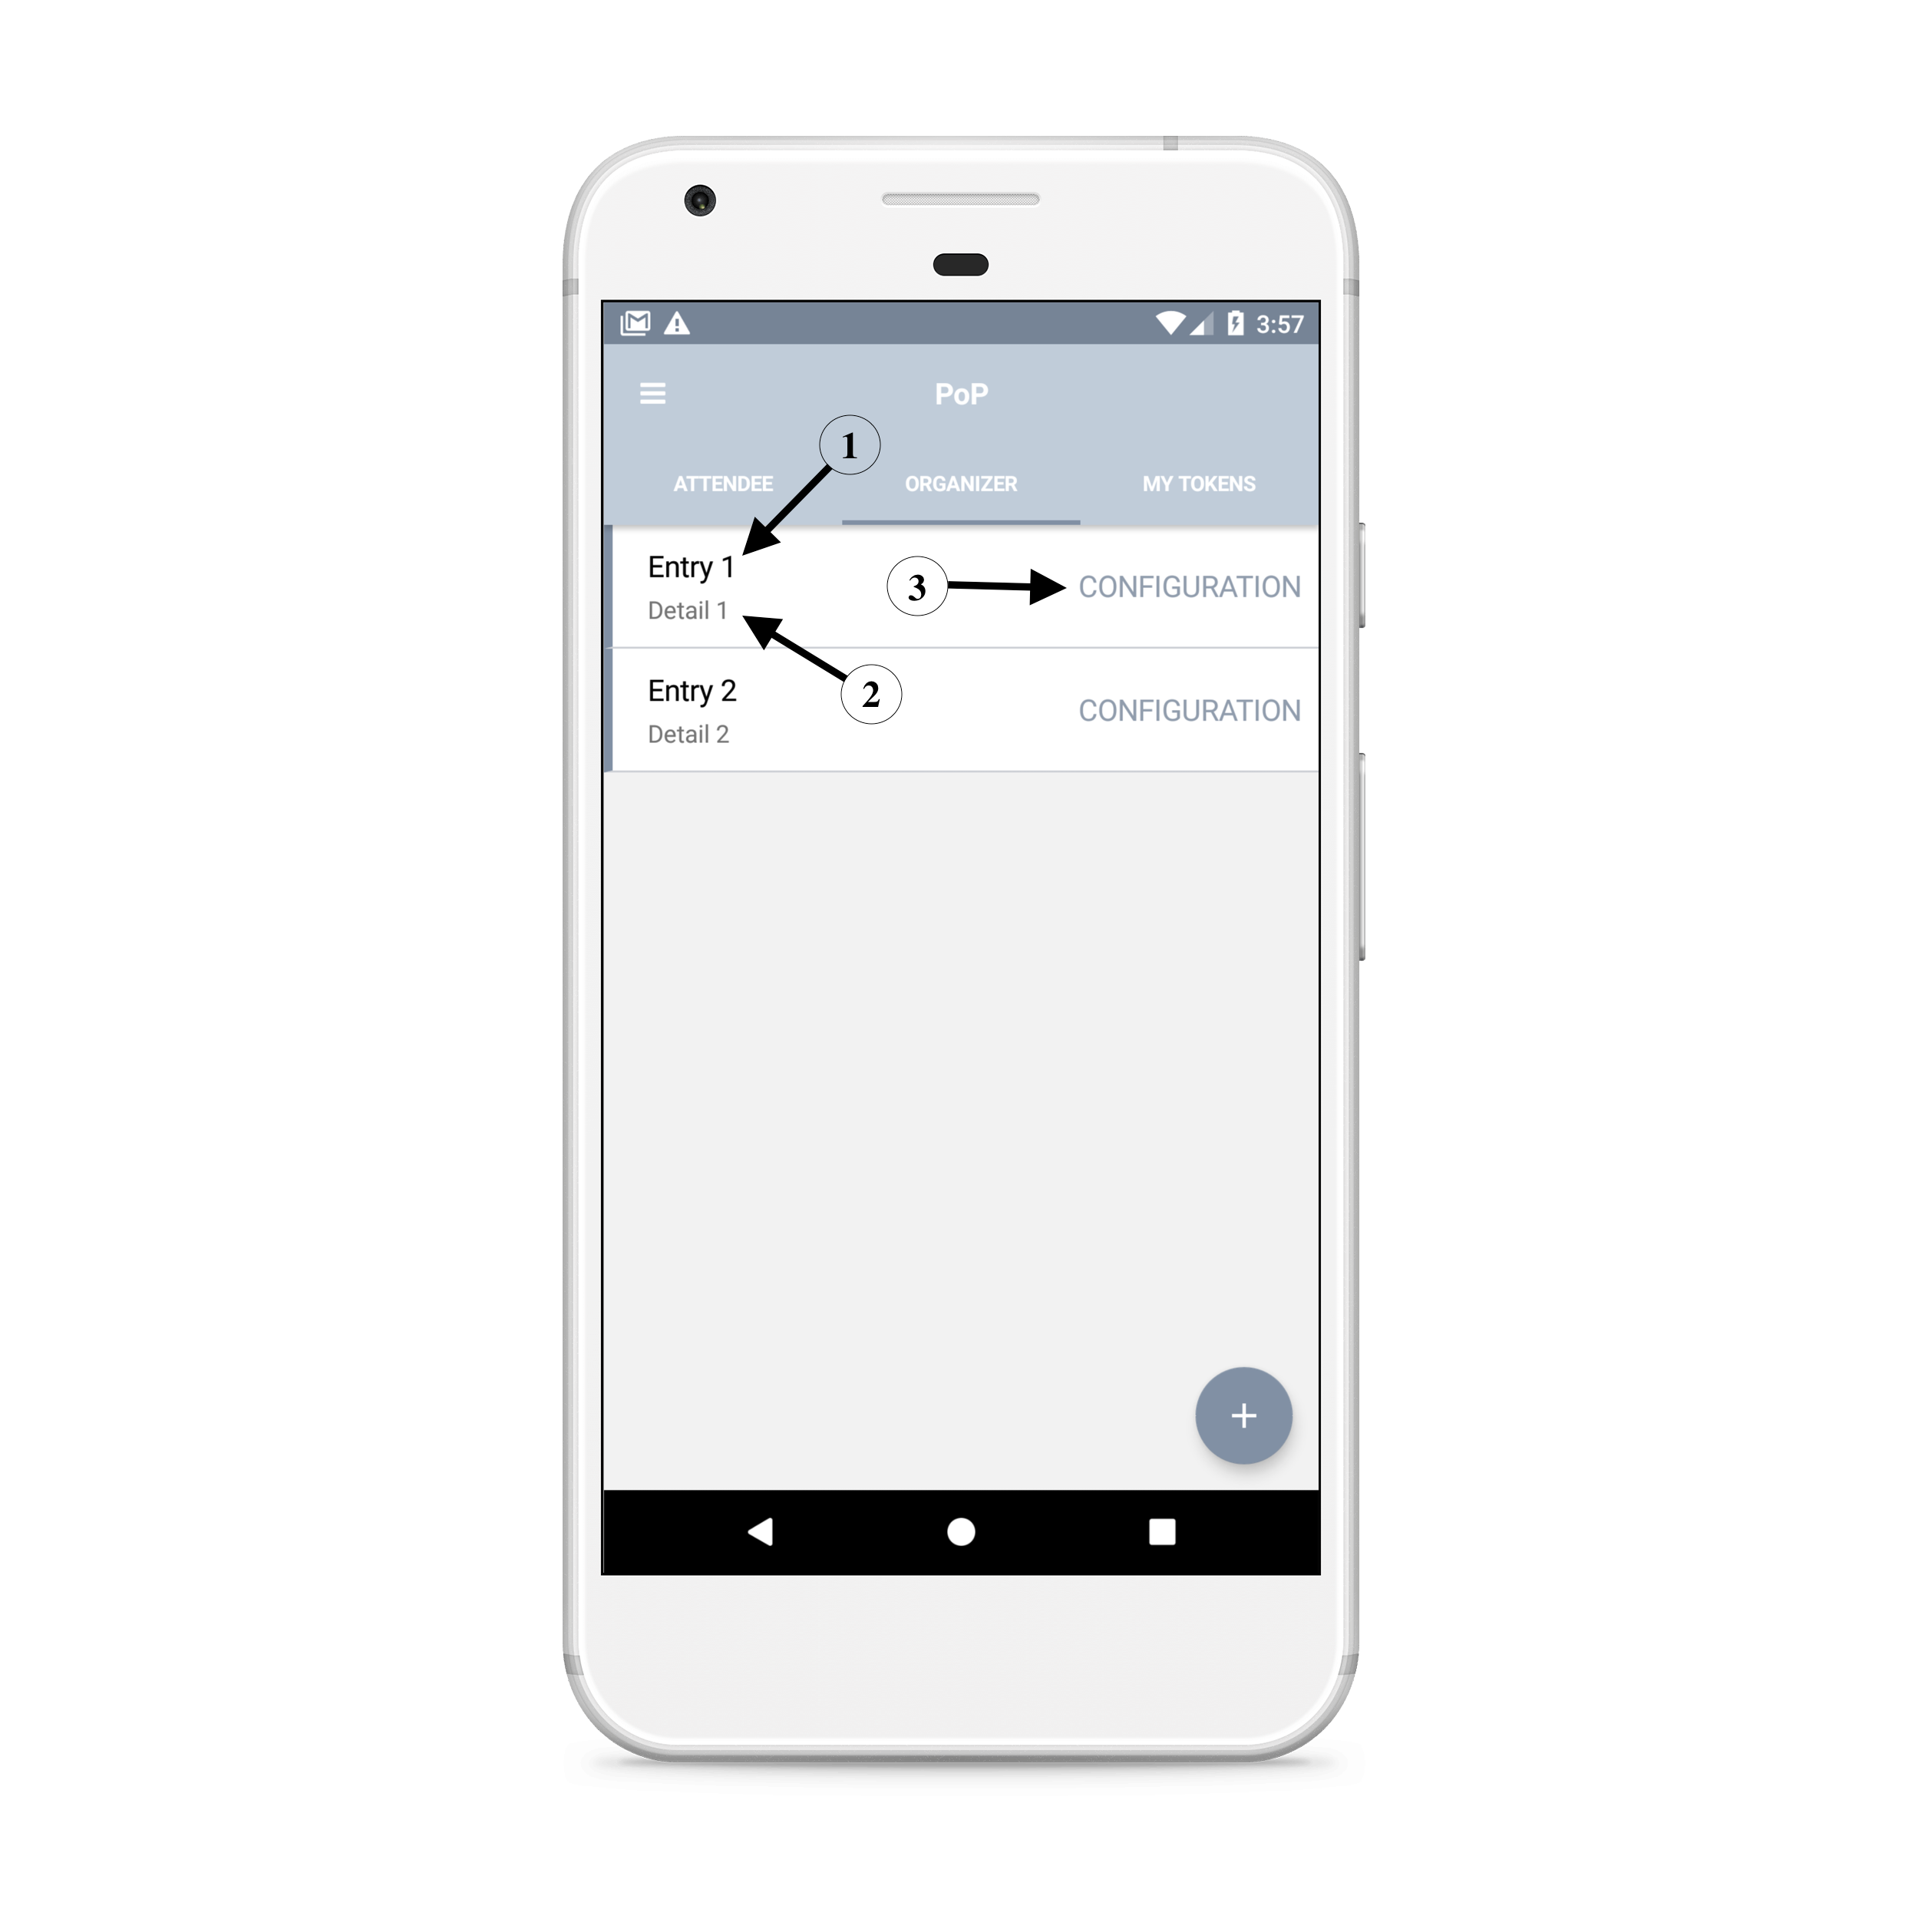
\includegraphics[height=0.8\linewidth]{resources/list_ui.png}
	\caption{Example of a typical list in CP-MAC}
	\label{fig:list_ui}
\end{figure}

\subsection{QR Code Presentation}
The modal page that presents a QR code to other users has also been updated. As this page is frequently used (a lot of information is exchanged by this medium, especially for the Proof-of-Personhood part), a special attention has been ported to create a nice-looking page. The result can be seen on Figure \ref{fig:qrcode_ui} at page \pageref{fig:qrcode_ui}.

\begin{figure}[!ht]
	\centering
	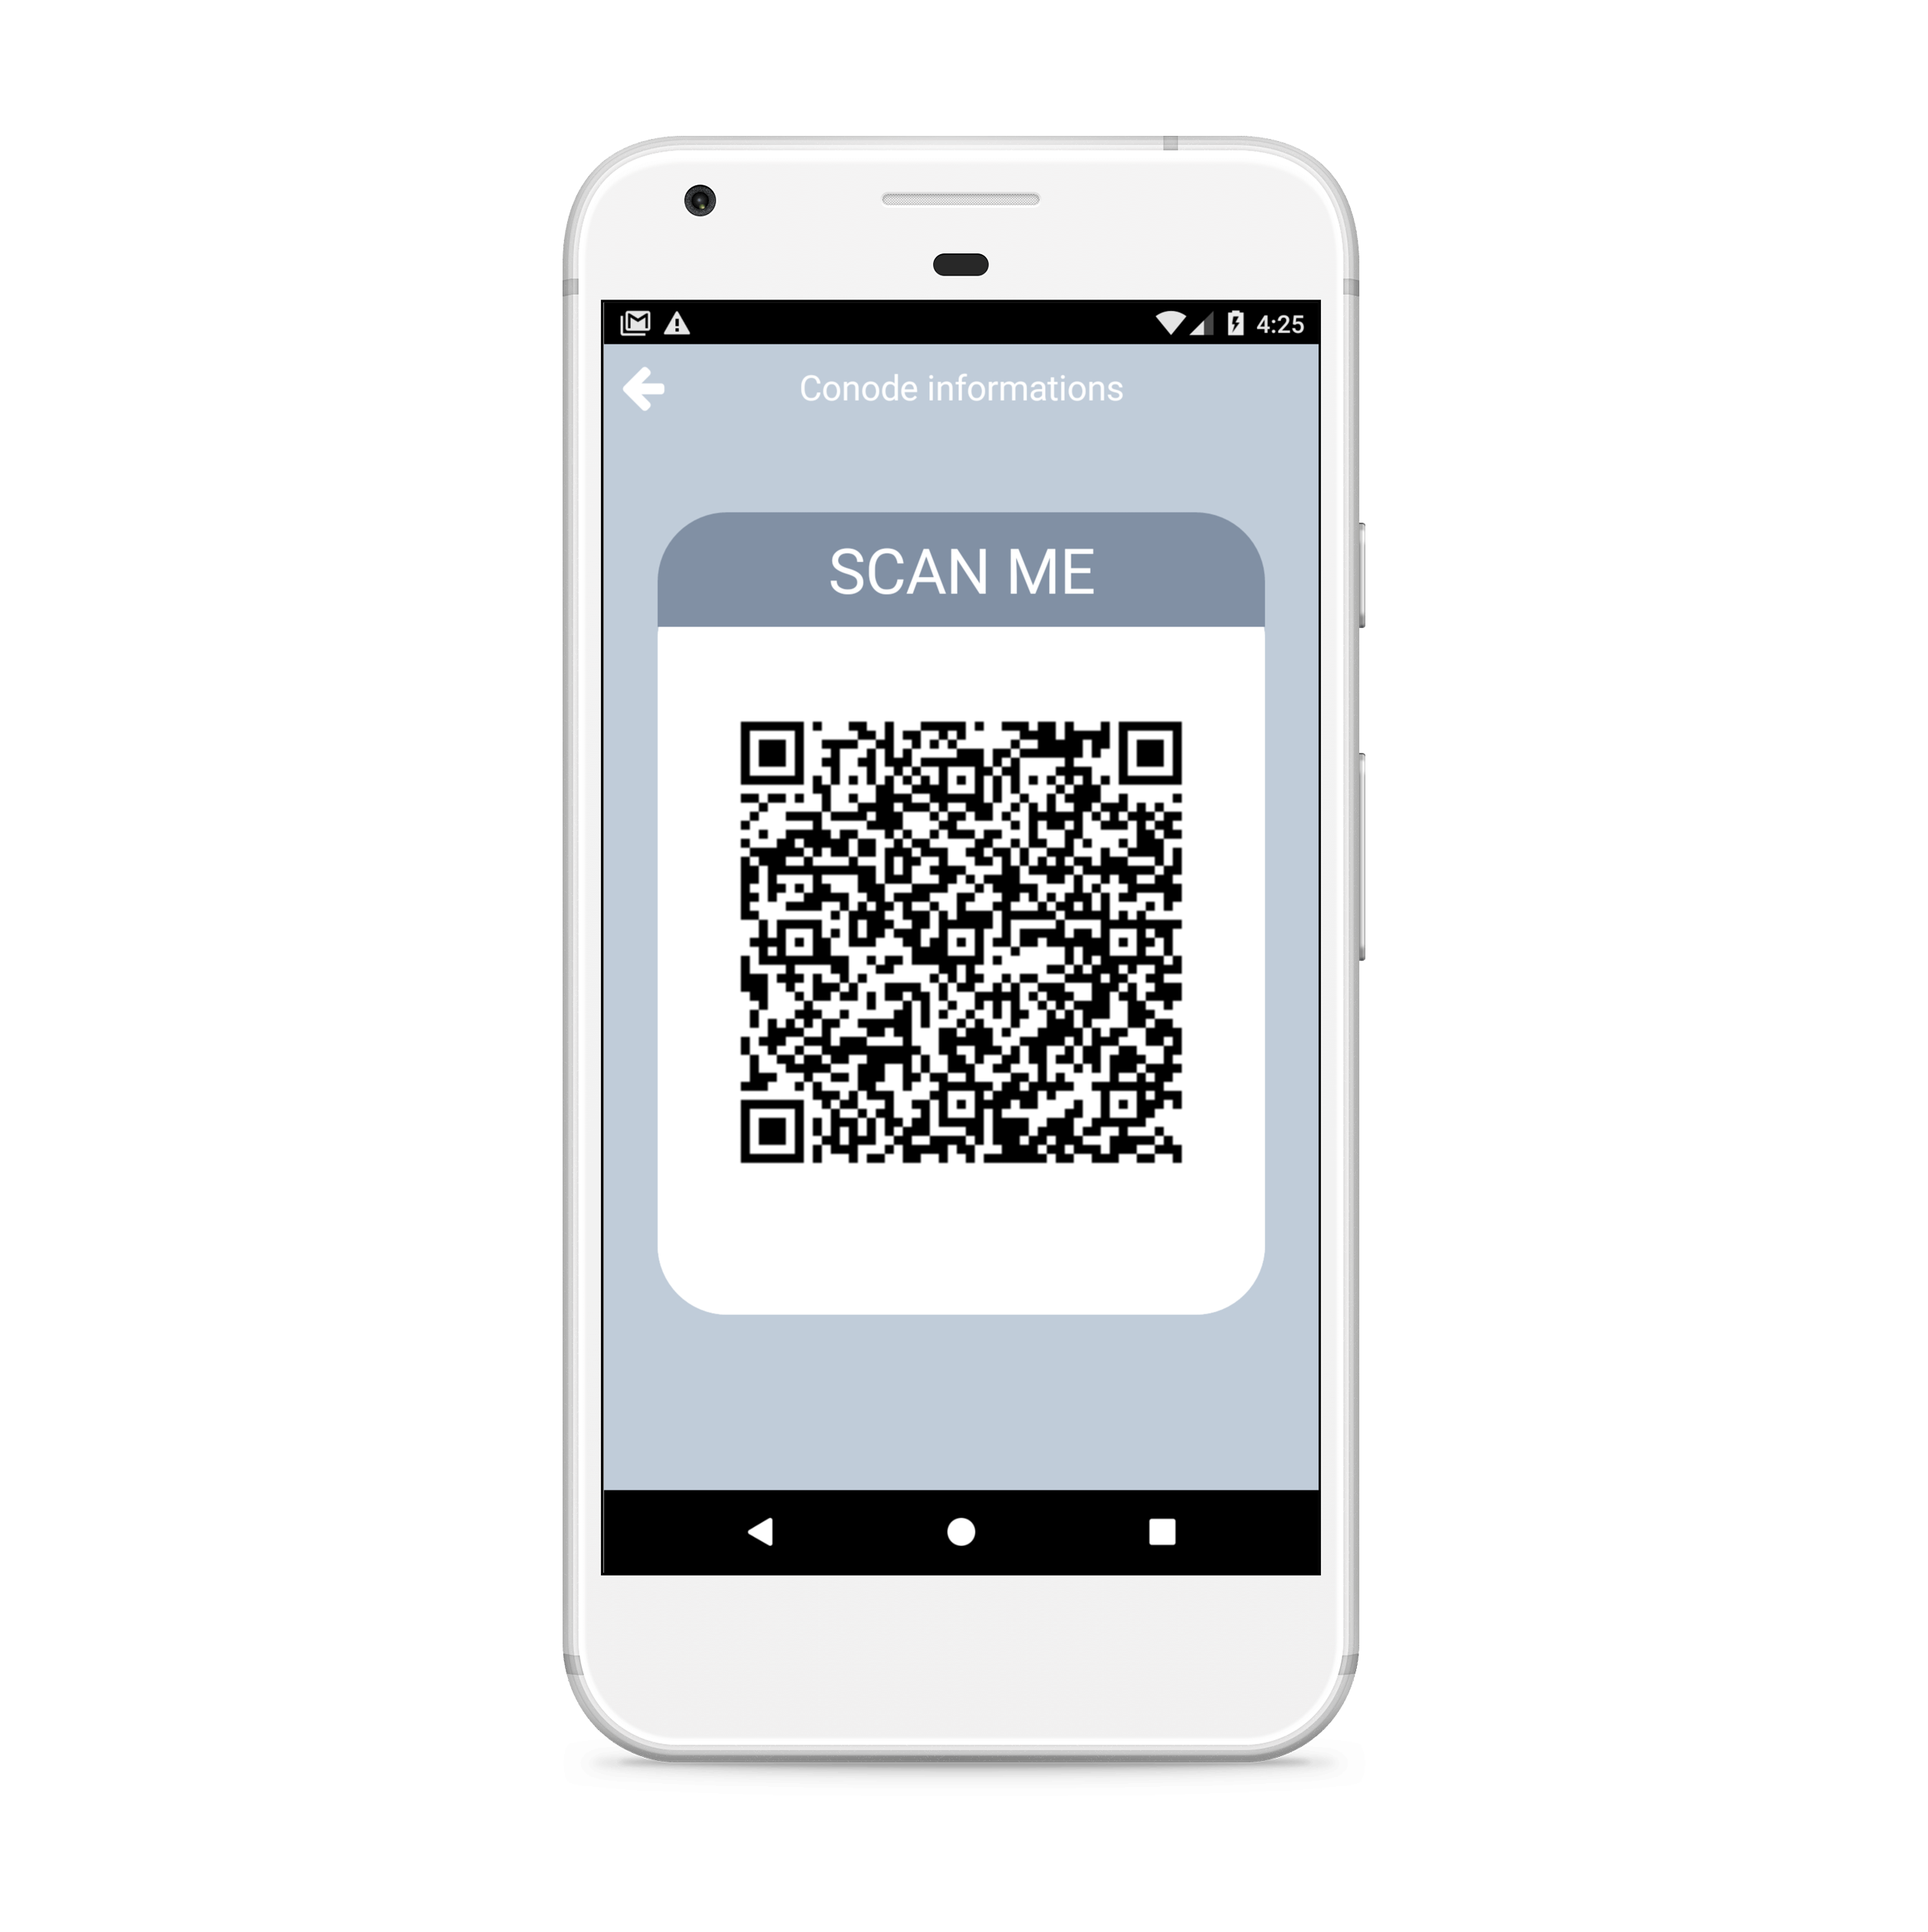
\includegraphics[height=0.8\linewidth]{resources/qrcode_ui.png}
	\caption{Example of the modal QR code presentation page}
	\label{fig:qrcode_ui}
\end{figure}

\chapter{PoP}

\paragraph{}
As already stated in the introduction, the backend for the PoP app is completely implemented in the Cothority framework, but it requires technical knowledge because one has to use the CLI to handle the functionalities. The first and main goal was to provide a user-friendly interface that is packaged in a cross-platform app for Android and iOS and allows anyone to use the technology provided by PoP. In this section, we describe the implementation of PoP in CPMAC and the process of creating, handling, and finalising a PoP party including the final PoP token creation.

\section{Implementation and Evaluation}

\paragraph{}
Three main classes form the PoP component: PoP.js, Org.js, and Att.js. The PoP.js object handles all information that is common or shared by the organiser and attendee status of a PoP party, for example the final statements and the PoP token the attendee owns. These are displayed in the PoP tab in the PoP drawer of the app. A final statement can be added by simply scanning a QR code provided by one of the organisers, deleting a final statement, generating a PoP token by linking it with the user’s key pair, and revoking PoP tokens to return to the final statement. When revoking a PoP token, the final statement is then restored, so the PoP token could now either be generated again by linking it with a key pair or the final statement can be deleted. This has been implemented so that the user can change the key pair linked to the PoP token if a mistake has been made.
The next class is Att.js, which, as mentioned previously, is only a skeleton for the class. At this point of development, this class is empty and acts only as a placeholder for future implementations that are specific to the attendee of a PoP party.

\paragraph{}
The last class is Org.js. This object is the most complicated one of the three as it has to handle every functionality that an organiser needs to create, handle, and finalise for a PoP party. The first step for an organiser is to link with a conode. This can be achieved by clicking on the corresponding button in the org tab in the PoP drawer. The organiser can then choose with which conode to link. The suggested conodes are the same ones registered in the home page. By clicking on the wanted server, the organiser is asked to enter a PIN (found in the server logs). If the correct PIN has been entered, the linked conodes name, description, public key, and ID are displayed in the org tab. This way, the conode to which an organiser last linked is always clear (but not a guarantee that the conode is still linked to the organiser). The displayed conode is the one that is contacted anytime a message needs to be sent. The next step is to fill in the configuration of the PoP party. This can be done by clicking on the corresponding button, which opens a new window. Then, it is necessary simply to enter the name, date, time, and location of the party. The last step of the configuration is to provide the roster so that the part can be hosted. Either the organiser can enter each conode manually or the QR codes of the other organisers can simply be scanned, which is the more convenient way to do it. Once the organiser has filled in the configuration, it can be easily shared with other organisers by displaying it as a QR code.

\paragraph{}
The process of sharing a PoP description could not be achieved using only a QR code, since the amount of data a code can contain is heavily restricted\footnote{\url{https://en.wikipedia.org/wiki/QR_code#Storage}}. Because of this restriction, we had to find a work around that permits organisers to share their configuration with other organisers. The current solution we propose is a third-party service called PasteBin\footnote{\url{https://pastebin.com}}. This means that when someone wants to share a configuration and displays the QR code, it is first uploaded to the PasteBin service. The QR code then displays the ID of the paste, and the other person , by scanning this code, then downloads the description from PasteBin. This solution is not ideal and should only be temporary until a better one can be implemented (see future works).

\paragraph{}
The other organisers could fill in the configuration too, but since they must be exact copies (the only exception is the order of the conodes in the roster), the description-sharing idea is highly recommended. Once all of the organisers have entered or imported the PoP party configuration, they have to save it on their respective conodes, which then returns an ID that should be identical for every organiser. After registering, the ID of the current PoP description is displayed in the org tab just under the currently linked conode and is now used for all subsequent actions. The next step is to register all of the attendees of the party. By clicking on the corresponding button in the org tab, a new window is displayed. On this page, the organiser can collect all of the public keys that should get registered. As always, either the public keys are entered by hand or it is possible to simply scan the QR code of the key pair. The order of the attendees is not important; however, organisers have to all register the same list of public keys as those that are not common to every conode are stripped out. Once all public keys are registered locally, they can be sent to the conodes by clicking on the register button (this finalises the PoP party on the respective conode). During this process, all organisers but the last one receives an error message that states that not all other conodes are finalised. Once the last organiser registers the attendees, everyone who received the error message can then return to the org tab and fetch the final statement by clicking on the corresponding button (the last one to finalise the PoP party automatically fetched it). By switching to the PoP tab, it should be possible to see the final statement. Organisers can now share this final statement with the attendees, and everyone can generate their PoP token by clicking on the final statement.

\paragraph{}
The process of linking to a conode and registering the PoP configuration (i.e., generating the ID of the party) are two crucial steps. During the linking process, the conode stores the public key of the organiser and then only accepts either messages that do not require a signature or signed messages that can be verified using this stored public key. The first signed message sent by the organiser is to register the PoP description. The ID is computed by hashing (in this paragraph, we always talk about SHA-256\footnote{\url{https://en.wikipedia.org/wiki/SHA-2}}) this description and the required signature along with the message in the ID signed using the Schnorr algorithm. The hash is computed by concatenating the strings of the name, date, time, and location and then appending the "aggregate" (point addition) of all of the public keys of the conodes that will host the PoP party. This forces the organisers to register exact copies of the party configuration (excluding the order of the conodes, thanks to commutativity). The second and last signed message sent by the organiser is the finalising request, which includes all registered attendees. The required signatures are the hash of the party ID concatenated with all of the public keys of the attendees. If either of the hashes are computed differently or signed using a private key that does not correspond to the public key stored on the conode, these messages are rejected.

\section{Results}

\paragraph{}
As of now, CPMAC is in its first development phase. The core libraries have been implemented, and currently only basic functionalities of CISC and PoP have been ported from the Cothority framework. For the PoP part, CPMAC enables anyone who wants to host or attend a PoP party to create, manage, attend, and finalise one. Moreover, it is possible to generate PoP tokens.

\paragraph{}
All of these functionalities have been implemented to be as user friendly as possible and should be more accessible to the public than the CLI that Cothority provided until now.

\section{Future Work}

\paragraph{}
As mentioned in the results section, only basic functionalities have been ported for now. However, all of the libraries and objects have been designed with the consideration that CPMAC will be extended by either providing CISC and PoP new functionalities or by even adding complete new Cothority apps like CoSi or Guard. Some possible future works are discussed below.

\begin{description}[style=nextline]
\item[Replacing PasteBin] The PasteBin service is currently used to share PoP configurations because they include too much data to be contained in a single QR code. This method relies on a third party, and it also exposes data (not sensitive, but still an undesirable situation) on the internet. In addition, it limits the number shares, as PasteBin only allows a certain number of pastes per 24 hours depending on the status of the user who created it (guest, member, pro). A solution that would lift all of these restrictions would be to implement a new fetch functionality directly into the PoP app of the Cothority framework. It is already possible to fetch the final statement from a conode with the knowledge of its ID, and thus the same procedure could be used to fetch the PoP description that corresponds to a certain ID. The new procedure would then require a first organiser to fill in the description, register it on that conode, and provide the others with the ID, and the remaining organisers would simply fetch the description from the first organiser’s conode and register it on their own.

\item[PoP Party Merging] It is possible for PoP parties to be merged. This means that people can organise multiple parties around the world and merge the final statements so that they are all considered as one single PoP party. This is useful if the generated PoP tokens should have the same proof value but people have to meet at different places.

\item[Viral PoP Parties] Once a PoP party is finalised, the final statement is registered on the hosting conodes. Moreover, all attendees listed in this statement are trusted people as they own a related PoP token. Attendees can then host a new PoP party on one of the hosting conodes using their PoP token as authentication (instead of linking to it by providing a PIN). This could ease the process of hosting PoP parties as an attendee without having to set up a conode.

\item[Sign and Verify Services] One of the main purposes of a PoP token is to be able to sign and verify different services. The token allows people to prove that they were at a certain location at a certain date and time, and thus it should provide some rights that were linked to the PoP party. As an example, we use the BeerToken suggested by the DeDiS laboratory. To begin, DeDiS would organise a PoP party and invite all of its members. The goal of the PoP party is to hand out PoP tokens called BeerTokens. A BeerToken would guarantee every attendee a free weekly beer at Satellite\footnote{\url{https://satellite.bar}}, the bar of EPFL. In order to make this possible, it would be required to either verify a BeerToken in order to know if the user has already ordered the one free beer of the week, or sign using a BeerToken to claim the weekly beer. All of this could be implemented in CPMAC by extending the core libraries and objects.
\end{description}


\section{Linkable Ring Signatures}
\label{sec:linkable_ring_signature}
Linkable ring signatures are the missing link in CP-MAC to make the PoP-Tokens useful. As stated before, they're necessary to sign data, but they are also required for the verification.  As this type of digital signatures is not available in KyberJS, it has been necessary to implement it directly in CP-MAC.

\subsection{Implementation}
The sign and verify algorithms are implemented in \textbf{RingSig.js}. It contains also every required auxiliary methods. The execution of the algorithm strictly follows the one implemented in the Kyber Go version and described in \cite{cryptoeprint:2004:027}.  However, as there are major differences between the Go language and JavaScript, some inner mechanisms had to be adapted.

First, as we saw in the BLAKE2 introduction at point \ref{subsubsec:blake2}, BLAKE2Xb is used by Kyber ring signature algorithm but is not available in KyberJS. Two approaches were considered, each one having their drawbacks :

\begin{description}[style=nextline]
	\item[Implement BLAKE2Xb for CP-MAC] As there are several modules in JavaScript that implement BLAKE2b, it is possible to create an instance of BLAKE2Xb without coding the complete algorithm, as a BLAKE2X function can be derived from any BLAKE2 instance (be it BLAKE2b or BLAKE2s). The procedure is described in \cite{aumasson2016blake2x}. This would have assured a complete compliance with the Kyber implementation. However, the remaining time available to complete this project wouldn't have allowed imple\-menting and testing it thoroughly, on top of adding the ring signatures feature.
	\item[Use another hash function] The nearest hash function that I could find is an implementation of BLAKE2Xs implemented in the StableLib\footnote{\url{https://github.com/StableLib/stablelib/tree/master/packages/blake2xs}}. As it provides the same capabilities than BLAKE2Xb, it can be used in ring signature as a replacement. However, the drawback of this solution is that it breaks the compatibility with the Go (reference) version of Kyber. Note that this drawback can be highly moderated by parameterizing the hash function in Kyber and KyberJS, as stated at point \ref{subsec:ring_sig_future_work}. Due to the lack of time, this solution has been chosen. 
\end{description}

The second change that had to be operated concerns the way Kyber marshals its data. This happens during the conversion of the cryptographic elements (points, scalars) to standard byte arrays. Kyber uses a DEDIS library called \textbf{fixbuf}\footnote{\url{https://github.com/dedis/fixbuf}} that allows a fixed length binary encoding of arbitrary Go structures. As there isn't an equivalent library from DEDIS for JavaScript, I implemented a method that reproduces the behavior of \textbf{fixbuf} specifically for ring signature structure. Effectively, here is the Go structure representing an unlinkable ring signature :

\begin{center}
\begin{lstlisting}[language=Golang, caption={Unlinkable ring signature structure}, label={code:ustruct}]
type uSig struct {
	C0 kyber.Scalar 	// generated during the signing process
	S  []kyber.Scalar 	// the length of S equals the number
						// of public keys in the anonymity set
}
\end{lstlisting}
\end{center}
and the one representing a linkable ring signature :
\begin{center}
\begin{lstlisting}[language=Golang, caption={Linkable ring signature structure}, label={code:lstruct}]
type lSig struct {
	C0  kyber.Scalar 	// generated during the signing process
	S  []kyber.Scalar 	// the length of S equals the number
						// of public keys in the anonymity set
	Tag kyber.Point 	// the tag, unique to the signer under 
						// the given scope
}
\end{lstlisting}
\end{center}
According to \textbf{fixbuf}, those elements will be marshaled and concatenated. This can be reproduced in CP-MAC, as KyberJS (like Kyber) allows mar\-shaling cryptographic elements and those structures only contains points or scalar. It's then sufficient to concatenate the resulting byte array of each element, in the right order.

With these changes in mind, the implementation has been done following these steps : first, a specific development version of Kyber for which the hash function is replaced by BLAKE2Xs has been compiled. Also, Kyber and KyberJS have been configured to use a deterministic random function, this way the results between each implementation of the ring signature algorithm can be compared. This facilitated the work as it allowed to verify at each step the coherence of the results.
\subsection{Unit testing}
The tests used to verifiy the \textbf{RingSig.js} implementation are the same as in the Go version, available in the \textbf{sig\_test.go} test suite. Particularly, three scenarios are tested. In each case, signature are tested against the correct and the wrong message, plus the tags are verified (length and validity) when applicable. Here are the different scenarios :
\begin{itemize}
	\item A trivial unlinkable signing process with a single member anonymity set is tested.
	\item An unlinkable signing process with a small anonymity set of three members is also tested. 
	\item  For linkable signatures, an anonymity set of three members is created and a scope is defined. The tags generated when verifying against the good message and a wrong one are then verified.
\end{itemize}
\subsection{Future work}
\label{subsec:ring_sig_future_work}
The most important goal for a future improvement is to make KyberJS fully compatible with Kyber, either by implementing BLAKE2Xb in JavaScript or by parameterizing the hash function. The latter would give a high degree of freedom: for example, it could be possible to create a new suite in Kyber that uses BLAKE2Xs as the hash function. KyberJS would then have to support parameterization of the hash function for a suite, which is currently not the case. However, the former solution have the advantage of being more efficient, as BLAKE2Xb is optimized for 64 bits processor, which begin to be the standard in today smartphones. Of course, by combining the two solutions, we get the best of both world.

\section{BeerCoin Part}
\label{sec:beercoin}
With the different primitives that are now available on CP-MAC, it is possible to create a real use-case. Here, it has been decided to realize a long-running joke at the DEDIS: the creation of a BeerCoin.

\subsection{Description}
The idea behind BeerCoin is that a group of people could each benefit from a free beer every month, week, or day at the expense of someone else. It's also important to preserve the anonymity of the members of the group. For example, it should not be possible to recognize a user from his signature, as well as deducing information about users between two periods. 

Concerning CP-MAC, it should be possible to create a bar from the application, with the possibility to define which group is allowed to get these BeerCoins, and the period before renewal. The bartender could then verify from CP-MAC if a user is allowed to have a beer, and the order history should be kept to allow the BeerCoin supplier to later pay his bill.

\subsection{Implementation}
To implement the BeerCoin, the PoP-Tokens have been used, because, combined with the linkable ring signature, they fulfill all the above require\-ments. Here is the way BeerCoin works in CP-MAC: at first, a user has to create a bar. He can select the group of people which will get the BeerCoins. To simplify this process, CP-MAC will present every group of people from the PoP-Parties in which the user was involved. In fact, when a party gets finalized (let it be an attendee party or an organizer party), the final statement is added to a \textit{bank}\footnote{This \textit{bank} of final statements is in fact the singleton defined in \textbf{PoP.js}, which was already implemented.} of final statements. This way, the user can easily choose for which group he wants to pay the beers. He then chooses a time period and a name for his bar, which concludes the configuration of the bar.

Right after the creation, the directory structure for a bar follows this schema :

\begin{center}
	\begin{minipage}[c]{0.5\textwidth}
		\dirtree{%
			.1 beercoin.
			.2 RANDOM\_UUID\_1.
			.3 bar\_config.json.
			.3 final\_statements.json.
			.3 checked\_clients.json.
			.3 order\_history.json.
			.2 RANDOM\_UUID\_2.
			.3 ....
		}
	\end{minipage}
\end{center}
As we can tell from the \texttt{RANDOM\_UUID} entries, the structure follows the same name generation than a \textbf{Party}\footnote{please refer to point \ref{subsec:pop_mult_parties} for more details.}. Also, here is the usage of each file :
\begin{description}
	\item[bar\_config.json] stores the bar information described above. It also stores the beginning date of the last period. If the difference between the current date and the last reset date is bigger than the defined period for this bar, the list of already seen clients should be reset, and the beginning date updated to reflect the current period.
	\item [final\_statements.json] stores the final statement linked to the party re\-presenting the group of people enjoying the BeerCoins. It will be used to verify the signatures of the clients.
	\item[checked\_clients.json] contains the list of the already seen clients. Their tags are saved in this list (see point \ref{subsubsec:bar_client_verif} for detailed explanations).
	\item[order\_history.json] contains the date of each order that still has to be paid. It can be emptied from the user interface, when all the beers have been paid.
\end{description}

\subsubsection{Client verification}
\label{subsubsec:bar_client_verif}
Once the bar is set up, the verification of a client is pretty straightforward: he first has to scan a QR Code containing the bar information, composed of a nonce and a linkage scope. The linkage scope must be unique for that period, as it will allow the bar to recognize if a client came twice in the same period. Hence, the linkage scope is generated as follows :
\begin{gather}
scope = bar\_name \Vert frequency \Vert year \Vert month \Vert day \\
frequency \in \lbrace daily, weekly, monthly \rbrace \nonumber
\end{gather}
For example, a bar called Satellite that offers a free beer every day for its members would generate the linkage scope \textit{Satellitedaily201868}, assuming the current date is June 8th 2018. The client now signs the nonce with his private key and the linkage scope. The bartender scans a QR Code containing the signature, which is then verified using the final statement public keys as the group of anonymity. If the resulting tag is already in the list of checked clients or if the signature is not valid, the bar refuses the order. Otherwise, the tag is added to the checked clients list, and a new order is logged in the history.

\subsection{Drawbacks and future work}
One of the drawback of this system is the combination of ring signatures with QR Code. Indeed, as we have seen in the listing \ref{code:lstruct} (page \pageref{code:ustruct}), one of the array size in the signature is proportional to the number of public keys in the anonymity set. However, QR Code maximal capacity is $2954$ bytes\footnote{\url{http://www.qrcode.com/en/about/version.html}}, which could be exceeded depending on the number of member in the group.

But is this limit really constraining ? Let's consider a real-world case: CP-MAC bar implementation use the \texttt{edwards25519} curve of KyberJS for the ring signatures. On it, points and scalars are marshaled to 32 bytes long arrays. Again, by referring to listing \ref{code:lstruct}, we can deduce the following inequality :

\begin{align}
	\label{eq:max_qr_pk}
	32 + 32 + 32*n = 32 * n + 64 &\leq 2954 \\
	\implies n &\leq 90.3125
\end{align}
where $n$ is the number of member in the anonymity set. 

From (3) we get that the maximum size of an anonymity set is 90. In CP-MAC, this wouldn't really be an annoying boundary, however, in a real-world situation, this could cause troubles.

A lot of new features could be thought for future work, such as integrating an in-app payment method, or even by allowing people to exchange BeerCoins as any other decentralized token. It could also be possible to work on the drawback explained above, for example by modifying the protocol and integrating a conode as intermediary. CP-MAC would then just serves as a control board, while all the signing processes and signature exchanges are done directly between the client and the conode.

\chapter{Installation and Running of CPMAC}

\paragraph{}
We will now see how to install all required dependencies and how to compile, test and run the app. The following steps are:

\begin{enumerate}
\item Installation of Go Language

To be able to run the cothority framework you'll need the go compiler. Install it by following the official installation guide: \url{https://golang.org/doc/install} . The \url{GOPATH} environment variable has to be set by either following the official guide\footnote{\url{https://golang.org/doc/code.html#GOPATH}} or by running\footnote{Terminal restart needed.}:
\begin{lstlisting}
$ echo 'export PATH=$PATH:$(go env GOPATH)/bin'
>> ~/.bash_profile
\end{lstlisting}

\item Cothority Installation and Running of Conodes\footnote{\url{https://github.com/dedis/cothority}}

CPMAC is developped to run against the stable version 1.2 of Cothority. As stated in the \url{README.md} file on the GitHub page of the cothority framework, the version installed in \url{gopkg.in/dedis/cothority.v1} has to be used. The source code in this folder corresponds to the branch v1.2 located here: \url{https://github.com/dedis/cothority/tree/v1.2}. Clone the repository by running:
\begin{lstlisting}
$ go get -u github.com/dedis/cothority
\end{lstlisting}
Locate and enter the folder \url{gopkg.in/dedis/cothority.v1} in your \url{GOPATH}, you can then execute the following command to run three local conodes:
\begin{lstlisting}
$ ./conode/run_conode.sh local 3 5
\end{lstlisting}

\item Official NativeScript Tutorial\footnote{\url{https://docs.nativescript.org/start/quick-setup}}

It is recommended to follow the instructions on their official page, as it will always be up-to-date. But here are the main steps:
\begin{enumerate}
\item NodeJS Installation\footnote{\url{https://nodejs.org/en/}}

This can be done by downloading the installer on their home page. Always install a long term service (LTS) version as it is the supported version for NativeScript.

\item NativeScript CLI Installation\footnote{\url{https://www.npmjs.com/package/nativescript}}

This can be done by running the following command:
\begin{lstlisting}
$ npm install -g nativescript
\end{lstlisting}
If an EACCES error is returned at some point of the installation, re-run the last command with administrator rights. If EACCES errors are still returned, run the command again with administrator rights and the unsafe permissions parameter of NPM:
\begin{lstlisting}
$ sudo npm install -g --unsafe-perm nativescript
\end{lstlisting}

\item Android and iOS Requirements

Since it depends on your operating system (OS), follow the official tutorial\footnote{\url{https://docs.nativescript.org/start/quick-setup#step-3-install-ios-and-android-requirements}}. NativeScript provides scripts for Windows and macOS that will automatically setup most dependencies. It is still recommended to look at the advanced setups they provide to ensure that everything is correctly installed.

\item TNS Doctor

The last step is to check if all requirements are met, this can be done by running: \url{tns} \url{doctor}. If errors are returned, fix them before continuing.
\end{enumerate}

\item Editor

This step can be skipped if the goal is to only run the app but not to contribute to the project. In essence, any editor could be used. We recommend using Visual Studio Code\footnote{\url{https://code.visualstudio.com}} since it is the officially supported editor and provides an official plugin\footnote{\url{https://marketplace.visualstudio.com/items?itemName=Telerik.nativescript}} to integrate with NativeScript.

\item Install, Compile and Run CPMAC

Before going further make sure the conodes and an Android emulator or iOS simulator is set up and running. Clone the repository by executing:
\begin{lstlisting}
$ git clone https://github.com/dedis/
student_17_mobile.git
\end{lstlisting}
After entering the newly created folder \url{student_17_mobile}, test and run CPMAC by executing either one of the following commands:
\begin{lstlisting}
$ make clean-test-<platform>
$ make clean-run-<platform>
\end{lstlisting}
Where \url{<platform>} has to be replaced by either \url{android} or \url{ios}. This will install and compile all the needed libraries and test or run CPMAC. All subsequent tests and runs can be made by running:
\begin{lstlisting}
$ make test-<platform>
$ make run-<platform>
\end{lstlisting}
\end{enumerate}


\chapter{"Known Bugs"}

\paragraph{}
As it is relatively new, NativeScript still exhibits some unexpected behaviours for which we had to find solutions. We now discuss some know bugs that have been bypassed or are still problematic.

// TODO: LIST AND FORMAT

- Compressed Files (Android)
Some NPM libraries are shipped with compressed files that usually end with ".gz" and are also included in their non-compressed form.  Ex:

    file.min.js
    file.min.js.gz
    
\paragraph{}
Android interprets these as a same and single file, this means that at compilation time Gradle will throw a "duplicate resources" error. To bypass this bug, we automatically delete the compressed version(they are not needed at runtime)) before they get compiled. You can find the corresponding commands in the "prepare-hook.sh" bash script.

- The BroRand Library(https://www.npmjs.com/package/brorand)
BroRand is a JS library to generate random numbers. CPMAC makes indirectly use of BroRand through the EC library called elliptic(https://www.npmjs.com/package/elliptic). BroRand is not fully supported on the NativeScript framework and throws an error at execution time when trying to generate a random number. We bypassed this by adapting the problematic lines in such a way that it works with NativeScript. You can find the corresponding command in the "prepare-hook.sh" bash script and the modified code in the "brorand-fix" folder

- WebSocket Bug (iOS)
The websocket library for NativeScript does not work correctly when run on iOS. Currently we didn't find a way to correct this bug in any way. The used library is called "nativescript-websockets"(https://www.npmjs.com/package/nativescript-websockets). Basically, this library wraps native websockets libraries for Android and iOS in JS objects. It seems that the wrapper implemented by "nativescript-websockets" is working properly, but that either the underlying native Objective-C library, which is a slightly modified version of PocketSocket(https://github.com/NathanaelA/PocketSocket), or iOS itself is causing troubles. It seems that either PocketSocket or iOS is resending previous messages by concatenating it with some new data. Below are two sent messages and the corresponding received messages by a conode, they are displayes in byte and base64 format to be easily readable. We verified that the sent messages are properly passed down to the native library by the JS wrapper. The first message is an empty pin request, thus only contains the public key of the organizer and is correctly received by the conode. The second message, which now also contains the PIN printed by the conode is not received correctly. The received message is the first message concatenated by six zeros and then the beginning of the second message.

Sent
EiDLgkwNauV7pExX7QEpT3Zdu7z4nxWRnmRXdK9KvZnEfA==
18 32 203 130 76 13 106 229 123 164 76 87 237 1 41 79 118 93 187 188 248 159 21 145 158 100 87 116 175 74 189 153 196 124

CgY3NTIzMTMSIMuCTA1q5XukTFftASlPdl27vPifFZGeZFd0r0q9mcR8
10 6 55 53 50 51 49 51 18 32 203 130 76 13 106 229 123 164 76 87 237 1 41 79 118 93 187 188 248 159 21 145 158 100 87 116 175 74 189 153 196 124

Received
EiDLgkwNauV7pExX7QEpT3Zdu7z4nxWRnmRXdK9KvZnEfA==
18 32 203 130 76 13 106 229 123 164 76 87 237 1 41 79 118 93 187 188 248 159 21 145 158 100 87 116 175 74 189 153 196 124

EiDLgkwNauV7pExX7QEpT3Zdu7z4nxWRnmRXdK9KvZnEfAAAAAAAAAoG
18 32 203 130 76 13 106 229 123 164 76 87 237 1 41 79 118 93 187 188 248 159 21 145 158 100 87 116 175 74 189 153 196 124 0 0 0 0 0 0 10 6


\paragraph{}
As already stated before, we were not able to bypass or fix this bug. Here is a non-exhaustive list of what we already tried but didn't succeed:

// TODO: LIST

- Find another NativeScript library to replace "nativescript-websockets"
- Modifying "nativescript-websockets" to try to reset the message buffer and others
- Natively implement websockets by using the same PocketSocket version as "nativescript-websockets"
- Natively implement websockets by using a different native library called SwiftWebSocket(https://github.com/tidwall/SwiftWebSocket)


\clearpage
\printbibliography

\end{document}
